\documentclass[11pt]{article}
\usepackage[a4paper,margin= 2cm]{geometry}
\usepackage{graphicx}
\usepackage{caption}
\usepackage{subcaption}

\title{\LARGE{\bf{Task 3 - Root Finding}}}
\author{\Large{\bf{Kirtan Patel - AE19B038}}}
\date{}

\begin{document}

\maketitle 

\section{Introduction}
This week's Task is:\\
Given a function F(x), find a value x\textsubscript{i} for which F(x\textsubscript{i}) = 0. We will use a 3 methods to solve the problem. 
\begin{enumerate}
	\item Interval Bisection Method
	\item Newton-Raphson Method
	\item Secant Method
\end{enumerate}

\subsection{Interval Bisection Method}
This method is an algorithm to find a zero of a function by repeated bisection of an interval and determination of the subinterval where the zero must be found. It is simple and reliable, but relatively slow.The essence of the bisection method lies in the fact that the sign of a function f(x) changes on opposite sides of a root.

Consider an interval [a,b] and a function f that has different signs at the boundaries of that interval: \[f(a).f(b)<0\]

Therefore, for a continuous function f, there must be atleast one zero within the interval [a,b]. To numerically approach a zero x\textsubscript{i} of f, the midpoint of the interval is taken as first approximation (with a1 = a , b1=b):
\[ c1 = a1 + \frac{b1-a1}{2} = \frac{a1 + b1}{2}\]

If the function value at the midpoint is still larger than the permissible error $\epsilon$, one has to repeat the bisection for the subiterval where the zero must be found. This can be determined from a change of sign of f,which can occur for one of the subintervals only (either for [a1,c1] or for [c1,b1]).\\

To determine which subinterval to continue the search in, we check the following:
\[if~~f(a1).f(c1)<0 \Rightarrow a2=a1, b2=c1\]
\[if~~f(b1).f(c1)<0 \Rightarrow a2=c1, b2=b1\]

In this new interval, we again determine the midpoint \[c2 = \frac{a2+b2}{2}\] and check the error at this point. \\

Continue this till we find a midpoint(root) which has an error less than the permissible error.\\
We can even set an upper-bound on the number of times we bisect the interval.\\

The code applied in the task takes both the above mentioned values as input and stops at whichever condition is met first.


\begin{figure} [h!]
	\centering
		\centering
		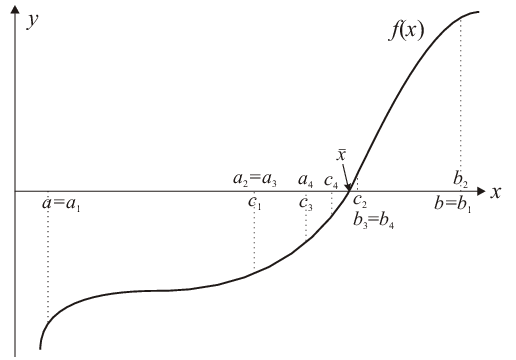
\includegraphics[width=0.5\linewidth]{bsm1}
		\caption{Graphical Representation of Root Finding using Interval Bisection Method}
		\label{fig1}
\end{figure}

\subsubsection{Remarks}
\begin{enumerate}
\item \textbf {Non-detectable zeros}\\
The interval bisection method relies on a change of the sign of . However, might have a zero where the sign does not change, i.e. where the graph does not cross the axis but just touches it. Such a second-order zero cannot be found by the interval bisection method.
\item \textbf {Multiple zeros}\\
The interval bisection method always converges to a zero. However, the given range might have several zeros in it . This will not be noticed by the interval bisection method, which therefore will find only one of them — but it is not clear which one will be found.
\item \textbf {Numerical Stability}\\
To detect a change of the sign of , the interval bisection algorithm is formulated above in terms of a product of two function values. Since a zero of is approached, these values can become very small, so that their product may lead to numerical underflow. This can furthermore be confused with the case that accidentally the midpoint is the sought-after zero, i.e. not the product but already a single function value equals zero. A robust numerical implementation must take care of these possibilities and should not use products of function values.
\item \textbf {Numerical Accuracy}\\
In general, the best accuracy that can be reached for the value of the zero does not equal the machine precision. This is related to the influence of the limited precision of floating-point arithmetic. Because of that, only the relative error can be used as a measure of numerical accuracy. In other words, the machine precision determines the smallest relative error reachable. Specifying an for the relative error smaller than the machine precision does not make sense and should be prevented. \\
\item \textbf {Numerical Reliablity}\\
Additionally, not only the deviation with respect to the value might be of interest: It may happen that the function has a rather steep slope at the zero, so that despite of a small relative error, , a function value may occur that is still large. Therefore it is advisable to check this after a zero has been determined numerically. \\
On the other hand, if the function has a rather low slope at the zero, the interval of very small function values can be rather large, which implies that the problem of numerical underflow described in remark 3 above might occur already before the prescribed accuracy has been reached. Then, the algorithm will most likely exit with an unreliable value. Obviously, in such a case it does not make sense to specify too small an for the relative error.
\end{enumerate}



\pagebreak
\subsection{Newton-Raphson Method}
The Newton-Raphson Method is a simple algorithm to find an approximate solution for the root of a real-valued function f(x)=0. If the function f satisfies sufficient assumptions then after repeative steps the x\textsubscript{n+1} given by:\[x_{n+1} = x_n -\frac{f(x_n)}{f'(x_n)}\] will be a good approximation to the root.\\

We can set 2 control parameters to control the root search:
\begin{itemize}
	\item error $\epsilon$ \\
	If f($x_n$) $<$ $\epsilon$, then we stop the iterations
	\item N$\_$max \\
	If the number of iterations crosses an upper-bound, then we stop the iterations and print the answer
\end{itemize}
If either of the conditions is met, then the iterations are stopped and the root is printed

\begin{figure}[h!]
	\centering
	\centering
	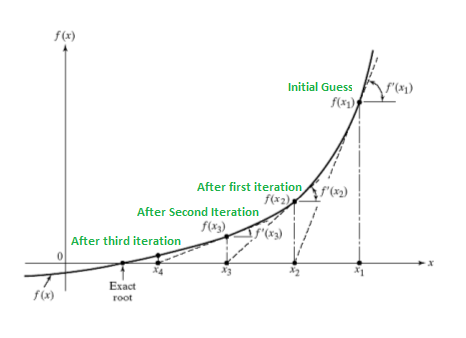
\includegraphics[width=0.8\linewidth]{nrm1}
	\caption{Graphical Representation of Root Finding using Newton-Raphson Method}
	\label{fig2}
\end{figure}
\vspace{1cm}
\subsubsection{Remarks}
Newton's method is only guaranteed to converge if certain conditions are satisfied. If the assumptions made in the proof of quadratic convergence are met, the method will converge. Failure of the method to converge indicates that the assumptions made in the proof were not met. 
\begin{enumerate}
	\item \textbf {Bad Starting Points}\\
	In some cases the conditions on the function that are necessary for convergence are satisfied, but the point chosen as the initial point is not in the interval where the method converges. In such cases a different method, such as bisection, should be used to obtain a better estimate for the zero to use as an initial point.
	
	\item \textbf{Iteration point is stationary}\\
	Consider a function \[ f(x) = 1 - x^2\]
	It has a maximum at x = 0 and solutions of f(x) = 0 at x = $\pm$1. If we start iterating from the stationery point $x_0 = 0$ (where derivative is zero), $x_1$ will be undefined, since the tangent at (0,1) is parallel to the x-axis.\\
	
	The same issue occurs if, instead of the starting point, any iteration point is stationery. Even if the derivative is small but not zero, the next iteration will be a far worse approximation
	
	\item \textbf{Starting Point enters a cycle}\\
	For some functions, some starting points may enter an infinite cycle, preventing convergence. Let  \[ f(x) = x^3 -2x + 2\]
	and take 0 as the starting point. The first iteration produces 1 and the second iteration returns to 0 so the sequence will alternate between the two without converging to a root. In fact, this 2-cycle is stable: there are neighborhoods around 0 and around 1 from which all points iterate asymptotically to the 2-cycle (and hence not to the root of the function).
	\item \textbf{Derivative Issues}\\
	There can be several issues related to the derivative of the function.If the function is not continuously differentiable in a neighborhood of the root then it is possible that Newton's method will always diverge and fail, unless the solution is guessed on the first try.
	
	Such cases include, derivative no being defined at the root and discontinuous derivatives.
	\item \textbf{Multiple Solutions}\\
	The algorithm found a solution but it does not mean that this solution is unique. Actually it found the closest. In case of multiple roots, it finds only one
\end{enumerate}
\pagebreak

\subsection{Secant Method}
The secant method is very similar to the bisection method except instead of dividing each interval by choosing the midpoint the secant method divides each interval by the secant line connecting the endpoints. The secant method always converges to a root of f(x)=0 provided that f(x) is continuous on [a,b] and f(a).f(b)$<$0.\\

The secant method procedure is almost identical to the bisection method. The only difference it how we divide each subinterval.

With an initial interval satisfying the initial conditions(a1=a, b1=b), we first compute f($x_o$), where $x_o$ is given by the secant line \[ x_o = a_o - f(a_o).\frac{b_o - a_o}{f(b_o) - f(a_o)}\]

To determine the next subinterval [$a_1, b_1$]:
\[if~~ f(a_o).f(x_o)<0 \Rightarrow a_1=a_o, b_1=x_o\]
\[if~~ f(b_o).f(x_o)<0 \Rightarrow a_1=x_o, b_1=b_o\]

We then find $x_1$ using the secant line formula and repeat the following steps till we reach son interval [$a_N, b_N$] which returns the value $x_N$, the x-intercept of the Nth subinterval\\

Here too, we can set 2 control parameters as mentioned before.

\begin{figure}[h!]
	\centering
	\centering
	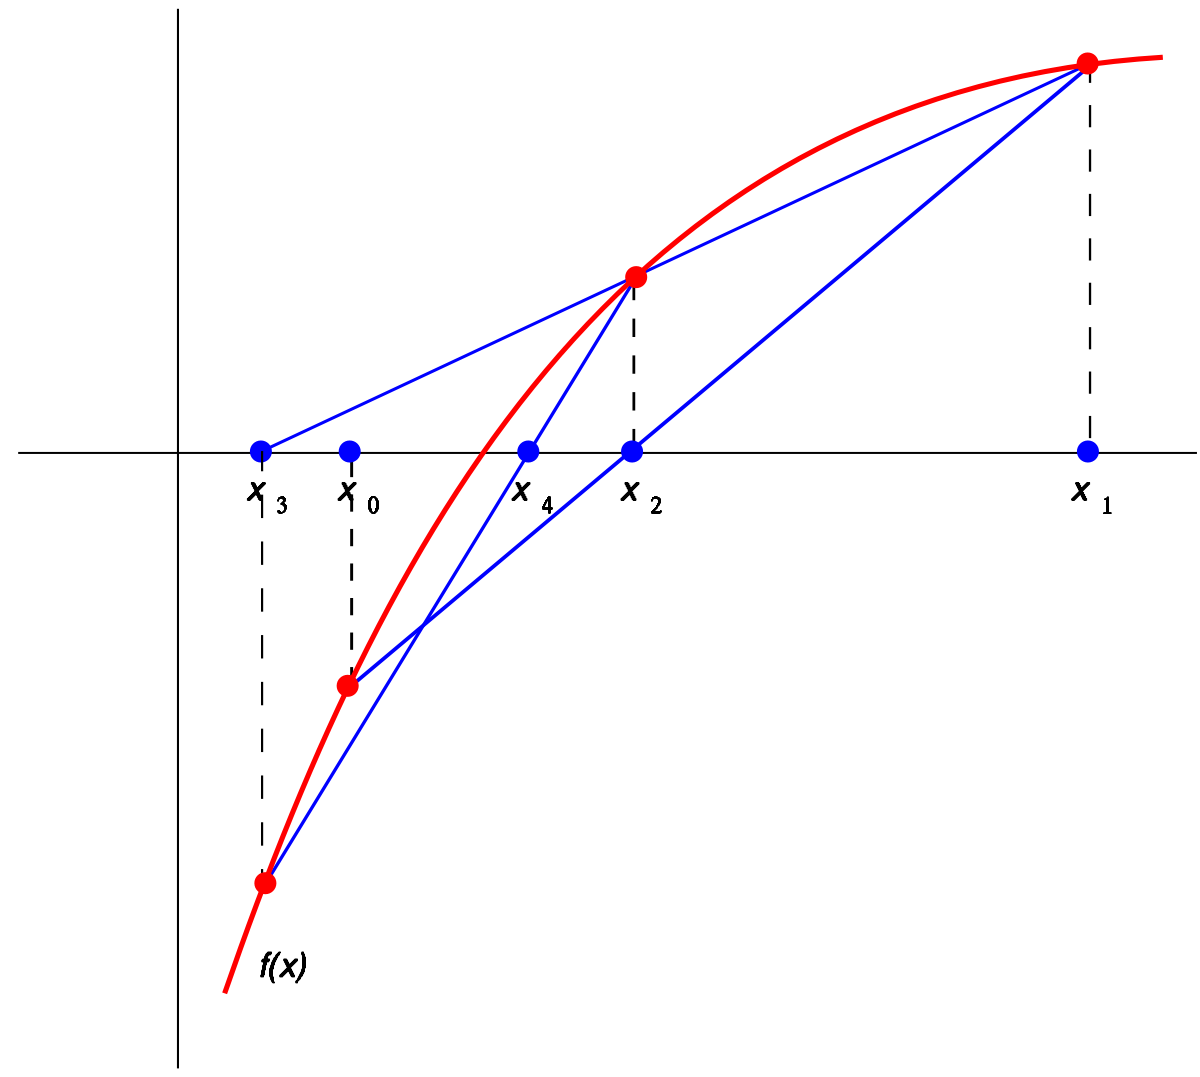
\includegraphics[width=0.6\linewidth]{secm1}
	\caption{Graphical Representation of Root Finding using Newton-Raphson Method}
	\label{fig3}
\end{figure}

\subsubsection{Remarks}
Secant Method is faster when compared to Bisection and Newton-Raphson methods as the order of convergence is higher in Secant Method. But there are some drawbacks too as follow:
\begin{enumerate}
	\item \textbf{It may not converge}
	
	\item \textbf{Derivative issues}\\
	It is likely to have difficulty if f´(a) = 0 i.e the x-axis is tangent to the graph y=f(x) at x = a.
\end{enumerate}

\section{Results and Analysis}
The following results are obtained by keeping the permissible error $\epsilon$ = 0.001, and varying the maximum number of iterations \textit{N} for different root-finding methods.

Here
\[ f1(x) = x^3 - 3x^2 - x + 9\]
\[ f2(x) = (x^3 - 3x^2 - x + 9).e^x\]

For each method, the results have been obtained for 2 sets of starting conditions. The below plots show the comparison between the results obtained.
\subsection{Interval Bisection Method}
\begin{figure} [h!]
	\centering
	\begin{subfigure}{0.55\textwidth}
		\centering
		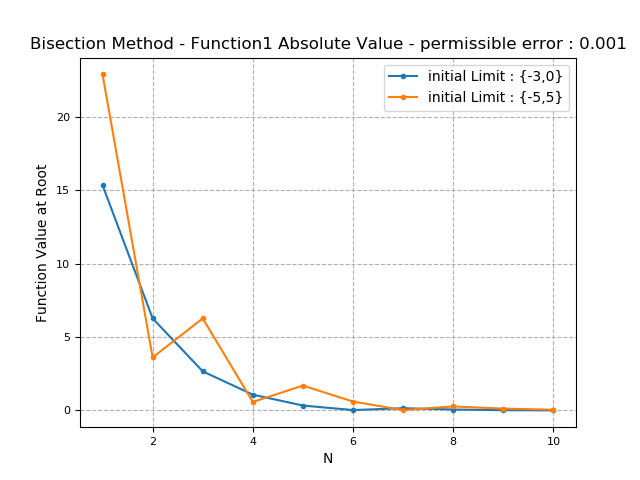
\includegraphics[width=\linewidth]{bsm-f1-abs}
		\caption{$\|$f1(x)$\|$ at the roots vs Max Number of Iterations}
		\label{fig1:sub1}
	\end{subfigure}%
	\begin{subfigure}{0.55\textwidth}
		\centering
		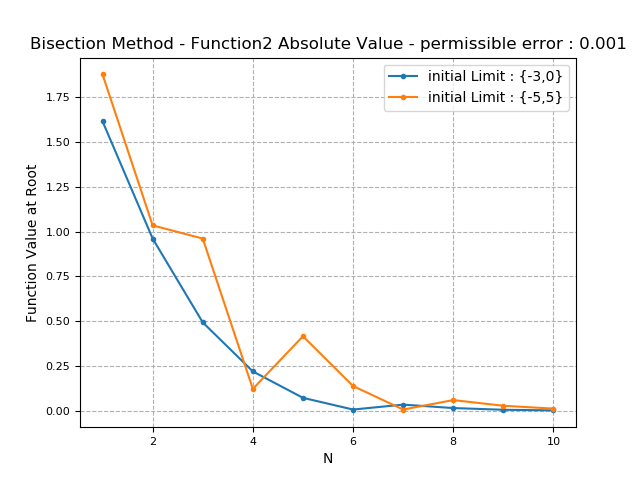
\includegraphics[width=\linewidth]{bsm-f2-abs}
		\caption{$\|$f2(x)$\|$ at roots vs Max Number of Iterations}
		\label{fig1:sub2}
	\end{subfigure}
	\caption{Results obtained using Bisection Method}
\end{figure}

\subsection{Newton-Raphson Method}
\begin{figure} [h!]
	\centering
	\begin{subfigure}{0.5\textwidth}
		\centering
		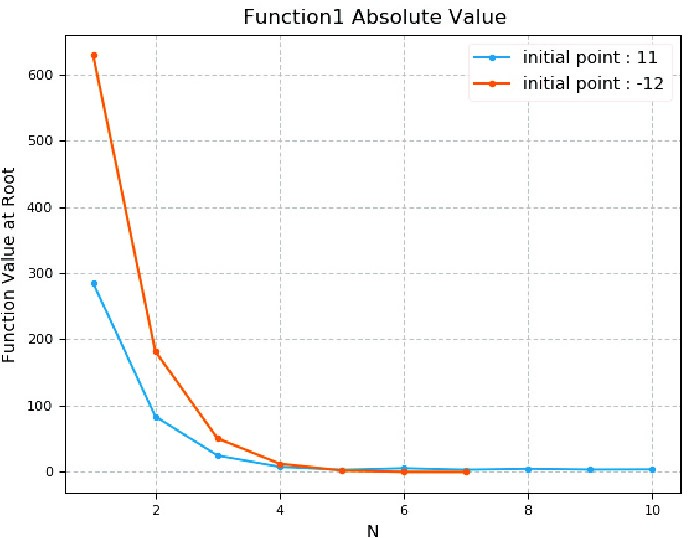
\includegraphics[width=\linewidth]{nrm-f1-abs}
		\caption{$\|$f1(x)$\|$ at the roots vs Max Number of Iterations}
		\label{fig2:sub1}
	\end{subfigure}%
	\begin{subfigure}{0.5\textwidth}
		\centering
		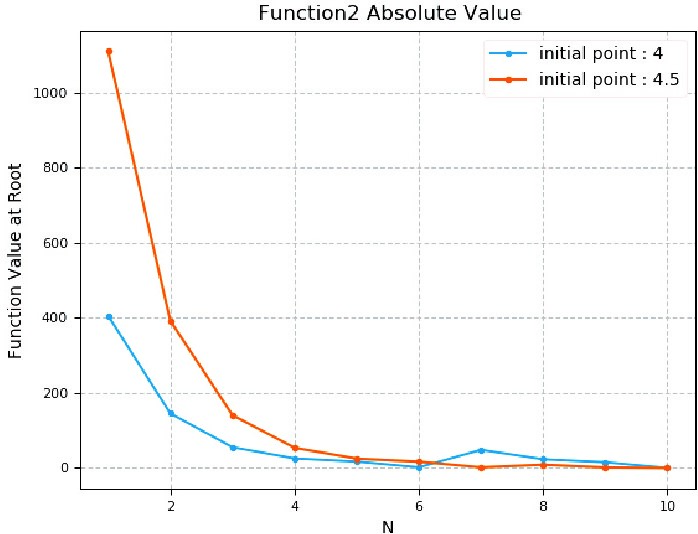
\includegraphics[width=\linewidth]{nrm-f2-abs}
		\caption{$\|$f2(x)$\|$ at the roots vs Max Number of Iterations}
		\label{fig2:sub2}
	\end{subfigure}
	\caption{Results obtained using Newton-Ralphson Method}
\end{figure}

\subsection{Secant Method}
\begin{figure} [h!]
	\centering
	\begin{subfigure}{0.55\textwidth}
		\centering
		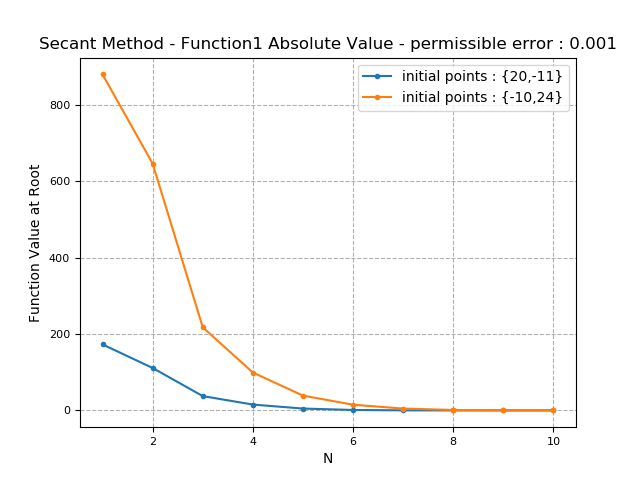
\includegraphics[width=\linewidth]{secm-f1-abs}
		\caption{$\|$f1(x)$\|$ at the roots vs Max Number of Iterations}
		\label{fig3:sub1}
	\end{subfigure}%
	\begin{subfigure}{0.55\textwidth}
		\centering
		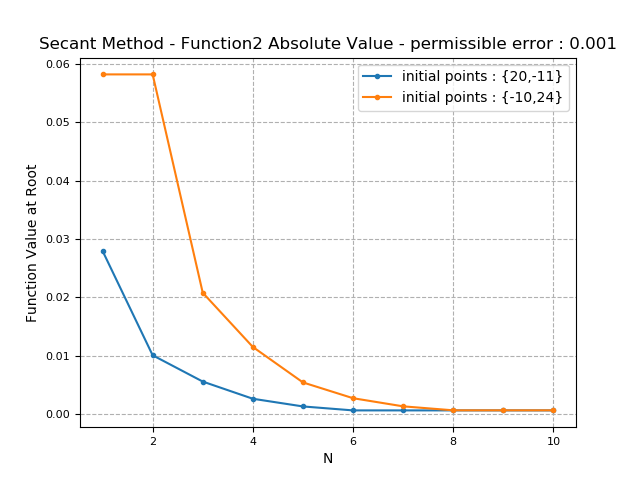
\includegraphics[width=\linewidth]{secm-f2-abs}
		\caption{$\|$f2(x)$\|$ at roots vs Max Number of Iterations}
		\label{fig3:sub2}
	\end{subfigure}
	\caption{Results obtained using Secant Method}
\end{figure}

\subsection{Comparison of Methods}
\begin{figure} [h!]
	\centering
	\begin{subfigure}{0.55\textwidth}
		\centering
		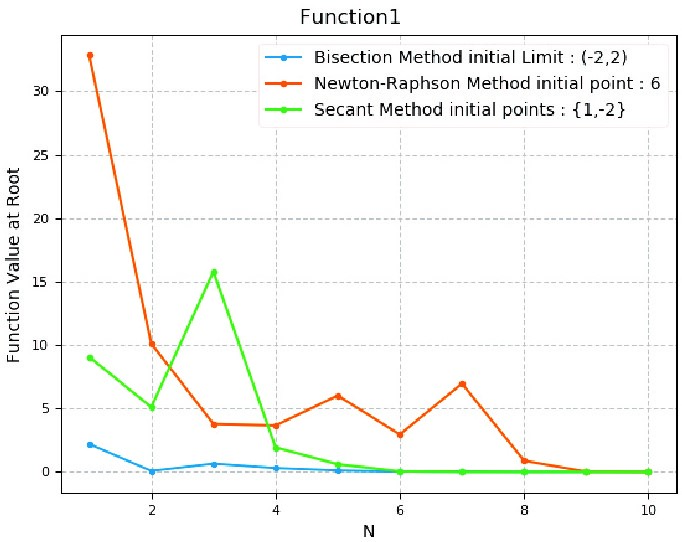
\includegraphics[width=\linewidth]{all-f1-abs}
		\caption{$\|$f1(x)$\|$ at the roots vs Max Number of Iterations}
		\label{fig4:sub1}
	\end{subfigure}%
	\begin{subfigure}{0.55\textwidth}
		\centering
		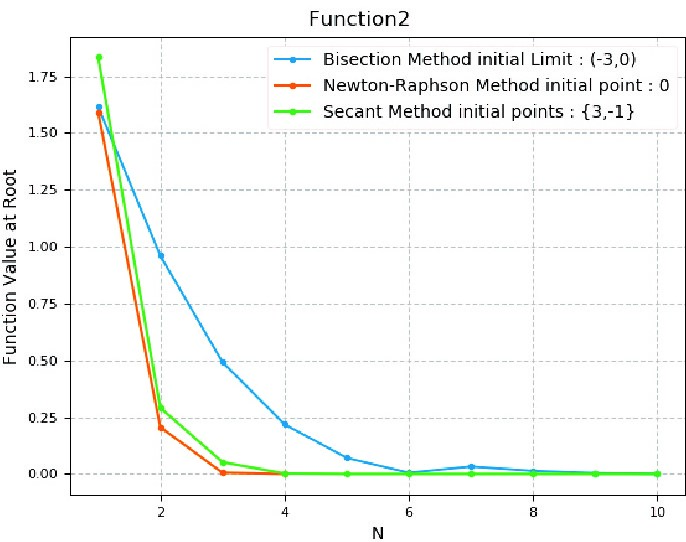
\includegraphics[width=\linewidth]{all-f2-abs}
		\caption{$\|$f2(x)$\|$ at roots vs Max Number of Iterations}
		\label{fig4:sub2}
	\end{subfigure}
	\caption{Comparison of Results obtained}
\end{figure}
\pagebreak
\section{Special Case}
Taking, \[f_3(x) = x^3 - 2x + 2~~~and~~~x_o = 0\]
using the Newton-Raphson Method to find the root, we get the following result.

\begin{figure}[h!]
	\centering
	\centering
	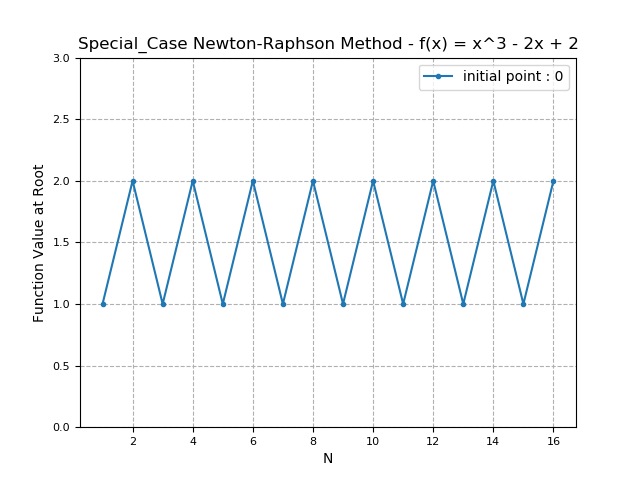
\includegraphics[width=\linewidth]{special_case_newton-raphson}
	\caption{Graphical Representation Special Case of Root Finding using Newton-Raphson Method}
	\label{fig4}
\end{figure}

Here we see one of the cases where the Newton-Raphson Method fails to converge to the root. The Starting Point is a part of a cycle.

Using,\[x_{n+1} = x_n -\frac{f(x_n)}{f'(x_n)}\] and the fact that \[f_3(x) = x^3 - 2x + 2 ~~ and ~~ f_3'(x) = 3x^2 - 2\]

For $x_o = 0$, f$_3$(0) = 2 and f'$_3$(0) = -2, and thus we get \[x_1 = 0 - \frac{2}{-2} = 1\]

For $x_1 = 1$, f$_3$(1) = 1 and f'$_3$(1) = 1, and thus we get \[x_2 = 1 - \frac{1}{1} = 0~~...\]
This cycle goes on and we are not able to obtain the root. This is mentioned in the section 1.2.1 .


\section{Inference and Conclusion}
It is very rarely the case that one particular method is better than another in all instances. Typically different methods have different strengths and weaknesses which make them good for some problems but bad for others. This is why in numerical analysis, we like to keep a broad range of tools in our toolboxes.\\

Consider, for example, a comparison of the bisection method and Newton’s method. When Newton’s method converges, it typically does so much faster than the Bisection method. We get the answer that we need with minimal computation, so it would seem that Newton’s method is better than the Bisection method. 

On the other hand, we need to remember that Newton’s method does not always work. Since the iterative formula involves a division by the derivative of a function, the method will completely fail if that derivative is 0 for any particular iteration. The nice thing about the Bisection method is that as long as you start with an interval that contains the root, you are guaranteed to converge! So with a problem that makes Newton’s method fail, Bisection is clearly a better alternative.\\

Evaluating the 3 methods of root-finding, we can see that while Bisection is very slow, it is always guaranteed to find a root once the process begins.
Compare this to Newton’s Method, which doesn’t have such guarantees.This is pretty typical behavior for the two algorithms since Bisection has linear convergence while Newton’s method quadratic convergence.

Bisection only requires function evaluations, but Newton’s Method also requires a first deriva-
tive. You may take this for granted in an academic setting, but in practical situations finding
the derivative can be impractical or expensive compared to a function evaluation. One way
to get around finding exact expressions for the derivative is to use a finite difference ap-
proximation for the derivative. The workaround is to use the Secant Method (Poor Man’s Newton Method), which approximates the derivative by the slope of a secant line. But this requires two starting guesses which are hopefully close to the root.\\

A more efficient method though is a combination of the two — simply, start with the bisection until you get a rough estimate of the root, then use Newton’s method to refine your estimate.\\


We can even tweak either of these methods to make them work better, and thus there are many more variations, but again, each has its own strengths and weaknesses.\\

\section{References}
\begin{enumerate}
	\item  https://x-engineer.org/undergraduate-engineering/advanced-mathematics/numerical-methods/the-bisection-method-for-root-finding/ 	
	\item https://silviaximenametodos.blogspot.com/2010/06/bisection-method$\_$29.html
	\item https://www.tf.uni-kiel.de/matwis/amat/comp$\_$math/kap$\_$1/backbone/r$\_$se19.html
	\item https://predictivehacks.com/newton-raphson-method-in-python/
	\item https://en.wikipedia.org/wiki/Newton's$\_$method
	\item https://www.quora.com/What-is-the-Newton-Raphson-method
	\item https://secure.math.ubc.ca/~pwalls/math-python/roots-optimization/secant/
	\item https://en.wikipedia.org/wiki/Secant$\_$method
	\item http://www.numericmethod.com/About-numerical-methods/roots-of-equations/secant-method
\end{enumerate}




\end{document}